
% !TEX root = ../UQML-main-handout.tex
% !TEX root = ../UQML-main-beamer.tex

\subsection{Theory of Importance Sampling}

% \begin{frame}[noframenumbering]
  \titlepage
\end{frame}

%%% Local Variables:
%%% mode: latex
%%% TeX-master: "UQML-main-handout"
%%% End:

\lecture{Introduction to Importance Sampling}{Intro-Importance-Sampling}

\begin{frame}{Monte Carlo Methods Review}

\begin{quote}
Monte Carlo Method is the art of approximating an expectation by the sample mean of a function of simulated random variables.\\
If $X$ is discrete:\\
\[\mathbb{E}(f(X))=\sum_{x \in \mathcal{X}} f(x) p_{X}(x)\]

If $X$ is continuous:\\
\[\mathbb{E}(f(X))=\int_{x \in \mathcal{X}} f(x) p_{X}(x) d x\]
\begin{flushright}
\textbf{}\\

\end{flushright}
\end{quote}
\end{frame}

\begin{frame}{Monte Carlo Methods}
Take the samples $X\sim p$ and we could have the Monte Carlo estimate:\\
\[\widetilde{f_{n}}(x)=\frac{1}{n} \sum_{i=1}^{n} f\left(x_{i}\right)\]
Notice that, $\widetilde{f_{n}}(x)$ is unbiased for $\mathrm{E}(f(X))$:\\
\[\mathbb{E}\left(\widetilde{f_{n}}(X)\right)=\mathbb{E}\left(\frac{1}{n} \sum_{i=1}^{n} f\left(X_{i}\right)\right)=\frac{1}{n} \sum_{i=1}^{n} \mathbb{E}\left(f\left(X_{i}\right)\right)=\mathbb{E}(f(X))\]
\end{frame}

\begin{frame}{Monte Carlo Method}

Monte Carlo Methods are widely used:

\begin{itemize}
\item Probability Approximation;\\
\item Simulate Distribution;\\ 
\item A Discrete Sum over Latent Variables.
\item $...$
\end{itemize}
Though Monte Carlo Methods are easy to formulate a quantity as an expectation, it is quite another thing to actually have the Monte Carlo estimator provide you with good estimates in a reasonable amount of computing time.\\
Typically, a \textcolor{red}{better} Monte Carlo estimator has smaller variance with the same computational effort than others.

\end{frame}

\begin{frame}{Pilot Example -- Probability of Cauchy Density}

\begin{quote}
Suppose that we are interested in the quantity of the probability $p$, which is a Cauchy $C(0,1)$ variable is larger than 2, described as the equation below:\\
\[
p(X>2) = \int_{2}^{+\infty }\frac{1}{\pi (1+x^{2})}dx
\]
Assume we can't integrate directly (of course we can use $arctan$ function) and we have to obtain $p$ by sampling the density.\\
What is the estimate and variance of estimator?
\begin{flushright}
\textbf{}\\

\end{flushright}
\end{quote}
\end{frame}

\begin{frame}{Different Estimators -- I and II}

\[
\boxed{
p(X>2) = \int_{2}^{+\infty }\frac{1}{\pi (1+x^{2})}dx}
\]

\begin{itemize}
\item I: The simplest model (naive sampling):\\ \[
\hat{p}_{1}=\frac{1}{m}\sum_{j=1}^{m}\mathbb{I}_{X_{j}>2}
\]
where, $X_{1}$ ,$...$ , $X_{n}$ $\sim$ $C(0,1)$ and i.i.d., and $\mathbb{I}$ is an indicator function. 
\item II: Taking into account the symmetric nature of $C(0,1)$:\\ \[\hat{p}_{2} = \frac{1}{2m}\sum_{j=1}^{m}\mathbb{I}_{\left | X_{j} \right |>2}\]

\end{itemize}
\end{frame}

\begin{frame}{Pilot Example -- Probability of Cauchy Density [1]}

\begin{figure}[ht]
		  \centering
          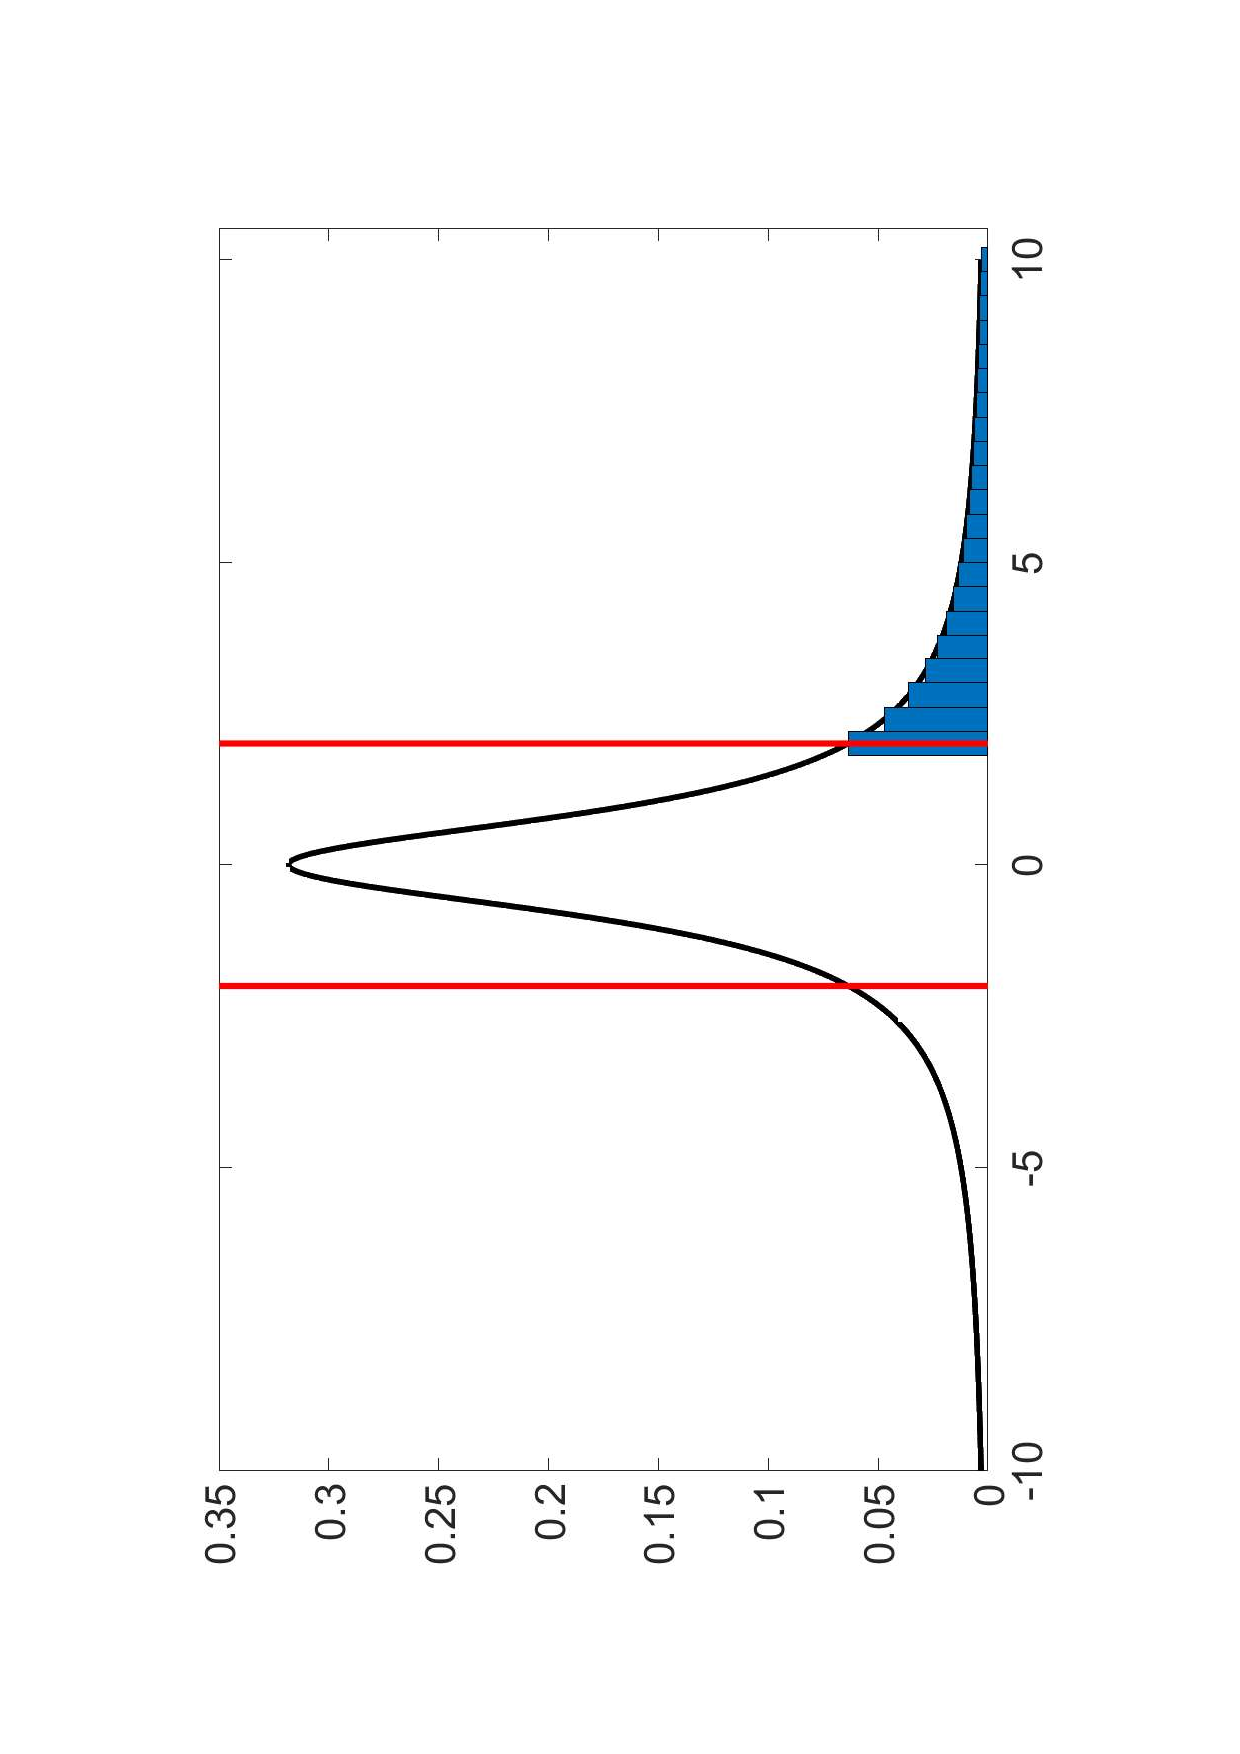
\includegraphics[scale = 0.3, angle = 270]{CauchyPDF12.pdf}
           \caption{Cauchy Distribution Estimator 1 and 2}
\end{figure}

\end{frame}

\begin{frame}{Different Estimators -- III}

\[
\boxed{
p(X>2) = \int_{2}^{+\infty }\frac{1}{\pi (1+x^{2})}dx}
\]

\begin{itemize}
\item The integral can be considered to be the expectation of :\\ \[h(X) = \frac{2}{\pi(1+X^{2})}\] \[\hat{p}_{3}=\frac{1}{2}-\frac{1}{m}\sum_{j=1}^{m}h(U_{j})\] \\ Where,  $U_{j}\sim \mathcal{U} {\left[ 0, 2  \right]}$ is a uniform distribution. 

\end{itemize}

\begin{alertblock}{Change of Measure}
The change of measure lead to a change of support from $[2, \infty]$ to $[0, 2]$. \alert{Why}?
\end{alertblock}

\end{frame}

\begin{figure}[ht]
		  \centering
          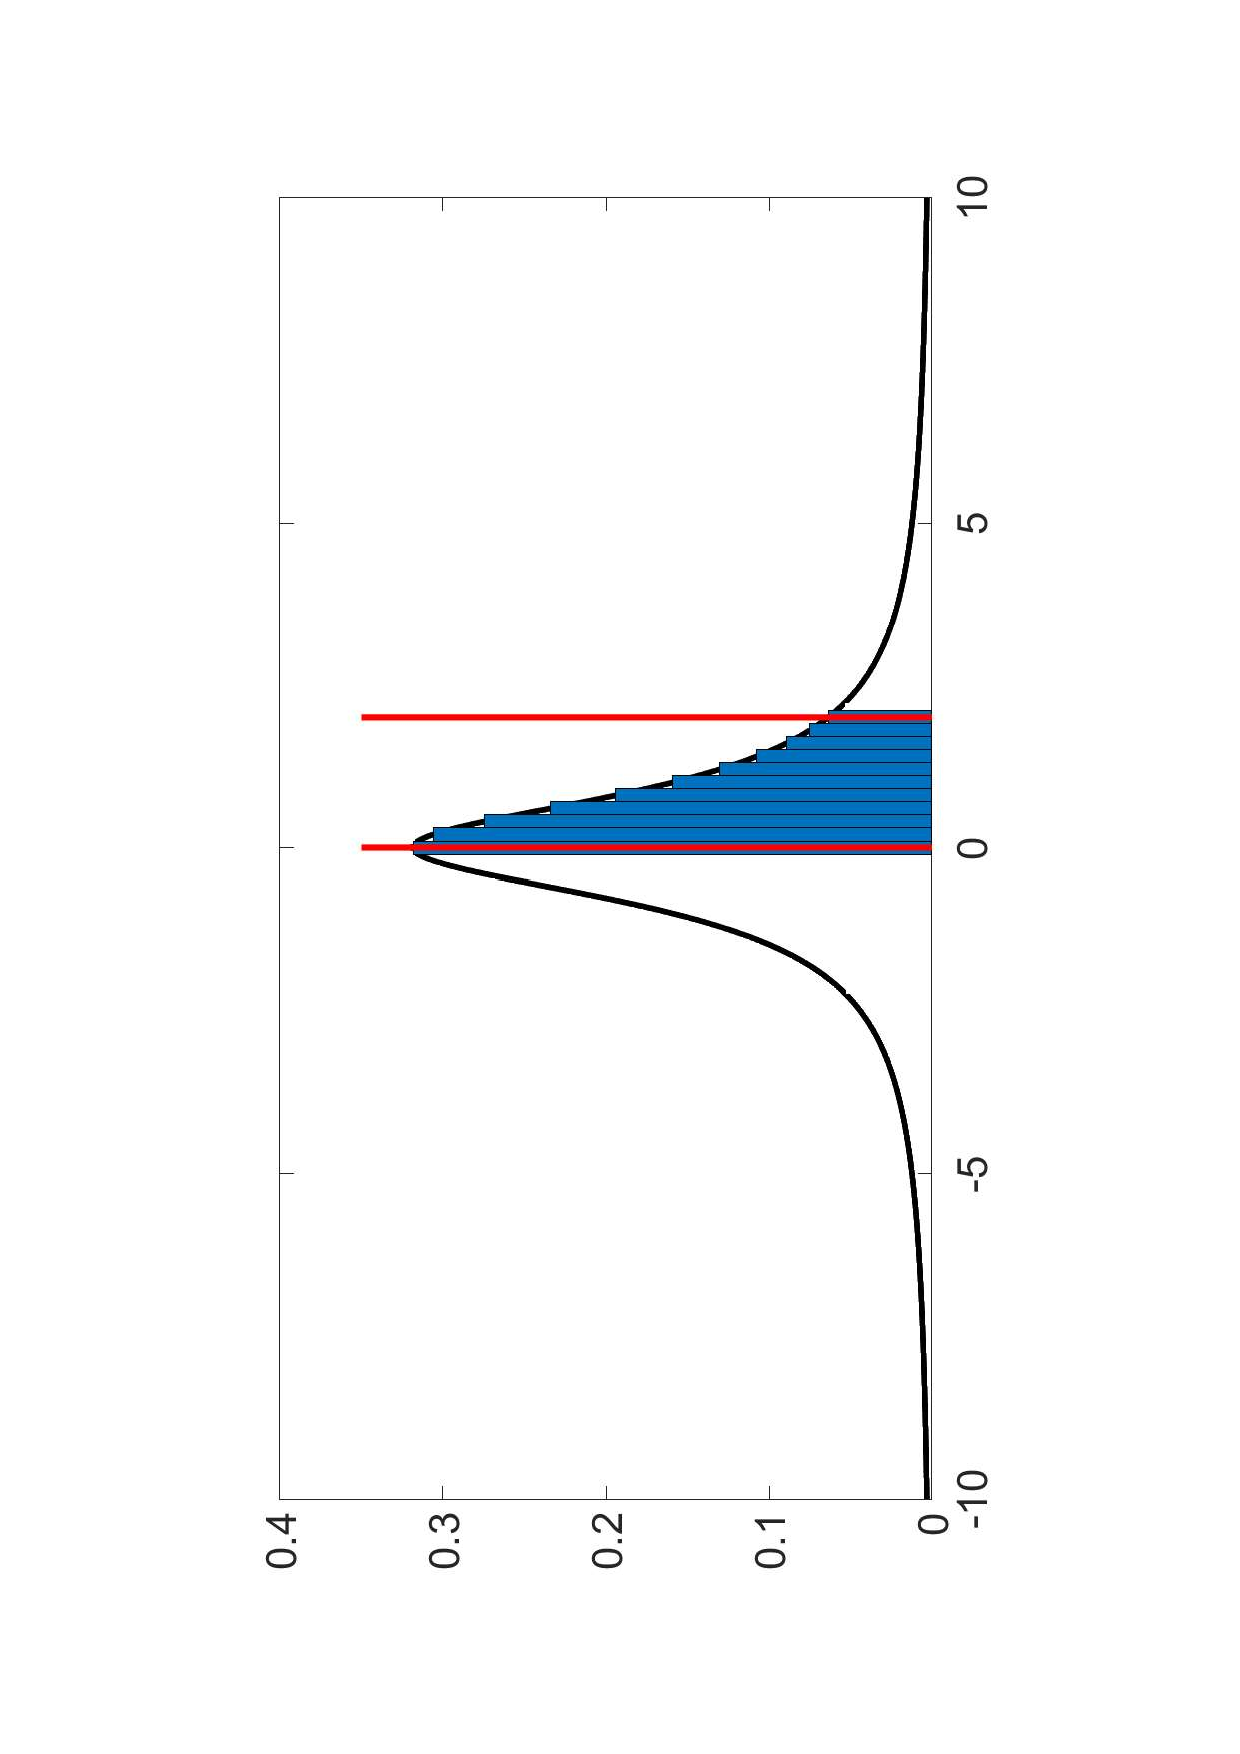
\includegraphics[scale = 0.3, angle = 270]{CauchyPDF3.pdf}
           \caption{Cauchy Distribution Estimator 3}
\end{figure}

\begin{frame}{Different Estimator -- IV}

\[
\boxed{
p(X>2) = \int_{2}^{+\infty }\frac{1}{\pi (1+x^{2})}dx}
\]

\alert{Change of measure from $p(x)$ to $p(y)$. Show!}

\begin{itemize}
\item Assume $y = x^{-1} $, the integral can be considered to be the expectation of:\\ \[h(Y) = \frac{2}{\pi (1+Y^{2})}\] \[\hat{p}_{4}=\frac{1}{4m}\sum_{j=1}^{m}h(Y_{j})\] \\ Where,  $Y_{j}\sim \mathcal{U} {\left [ 0, \right \frac {1}{2}]}$. 

\end{itemize}
\end{frame}

\begin{frame}{Pilot Example -- Probability of Cauchy Density}

\begin{figure}[ht]
		  \centering
          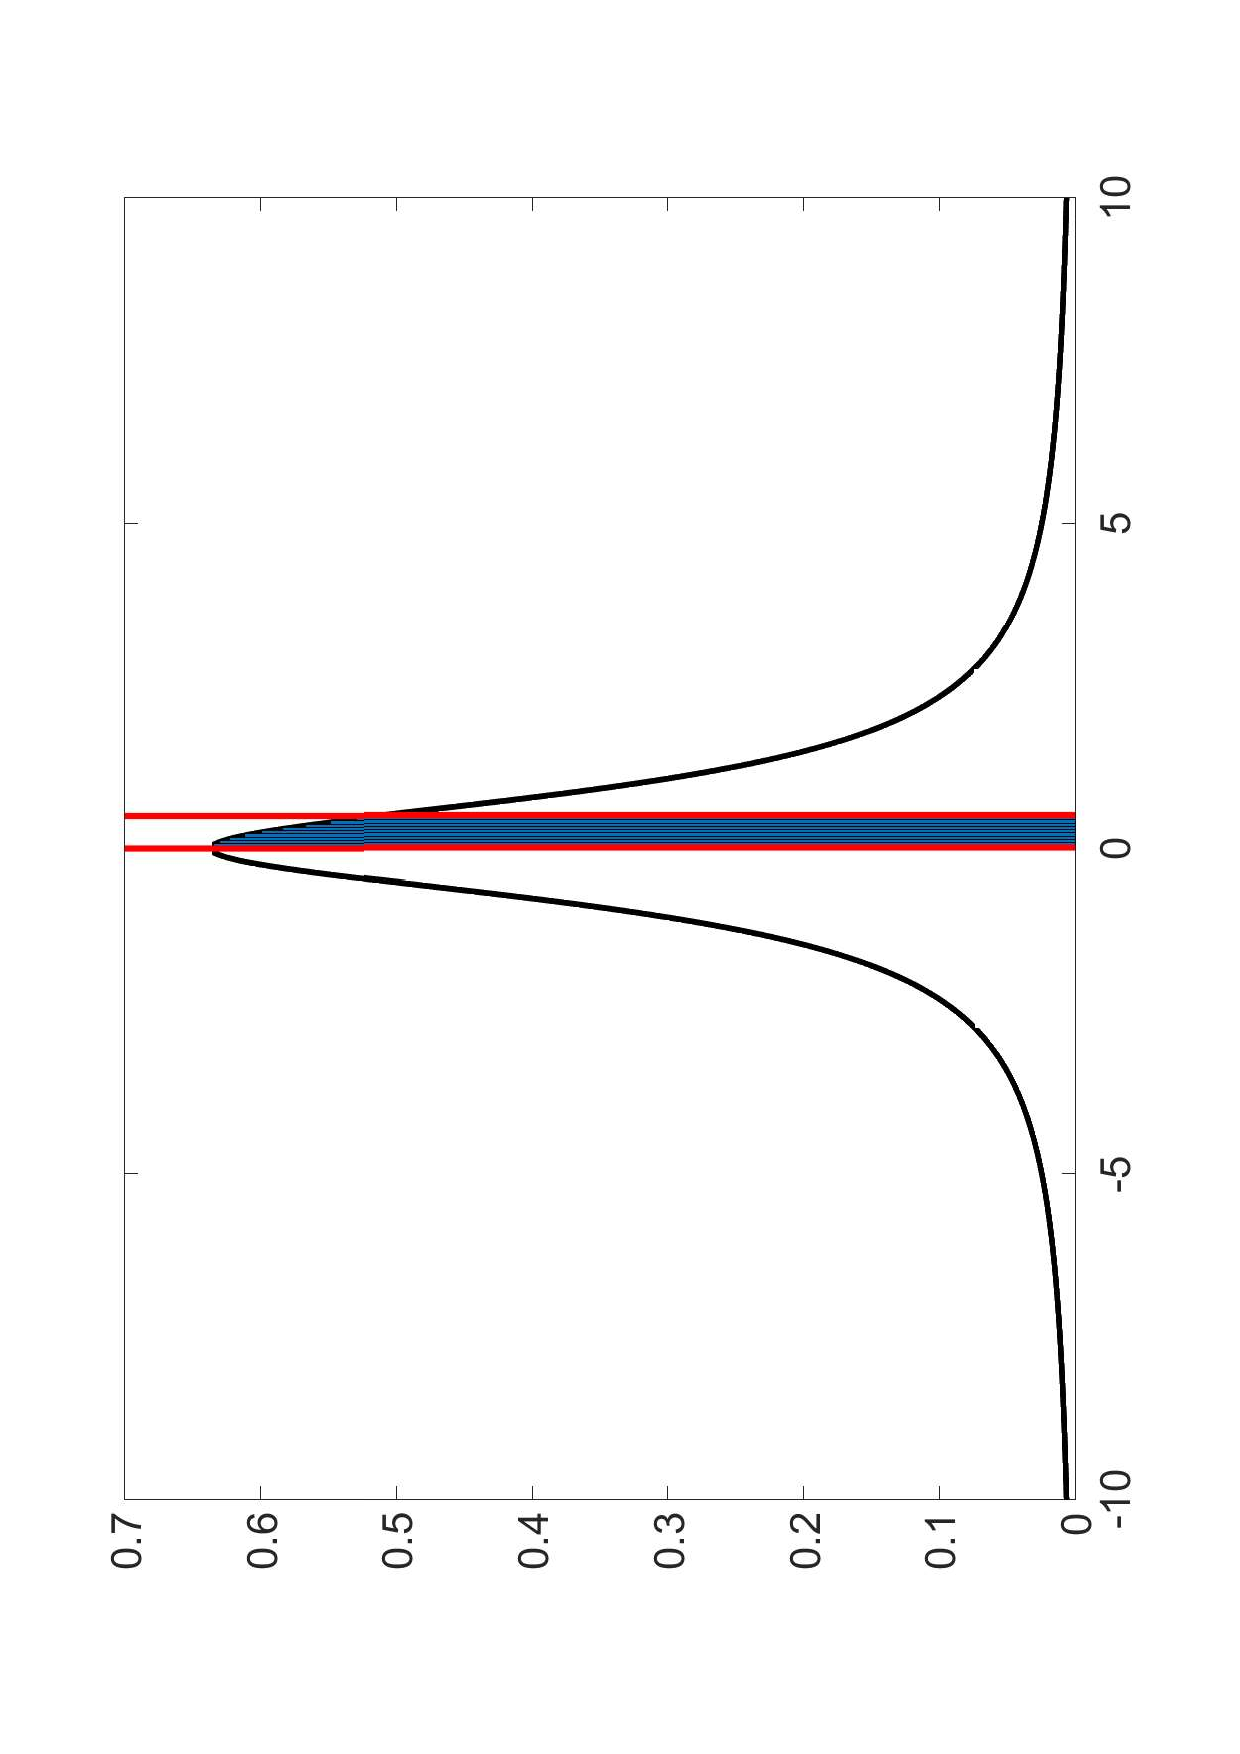
\includegraphics[scale = 0.3, angle = 270]{CauchyPDF4.pdf}
           \caption{Cauchy Distribution Estimator 4}
\end{figure}

\end{frame}

\begin{frame}{Variance}
\begin{columns}[c]
\column{1.0\fullcolwidth}
Question: \\
Under the same sampling size $m$, what is the variance of the estimator above?

\emph{Will they make big difference using different sampling method?}
\column{0\fullcolwidth}
\end{columns}
\end{frame}

\begin{frame}{Variance}
\begin{columns}[c]
\column{1.0\fullcolwidth}
The actual probability $p=0.1476$. According to the variance calculation of the Binomial distribution, the variance of Estimator 1, 2, 3 and 4 are $\frac{0.127}{m}$, $\frac{0.052}{m}$, $\frac{0.0285}{m}$, and $\frac{0.000095}{m}$ respectively ($m$ is the sampling size).\\
From estimator $\hat{p}_{1}$ to estimator $\hat{p}_{4}$, the variance reduction is of order $10^{3}$, which means that the sampling size of $\hat{p}_{1}$ should be $10^{6}$ times more than $\hat{p}_{4}$ to achieve the same precision (Monte Carlo integration error is proportional to $O(N^{-\frac{1}{2}})$.

\emph{What is an effective way to reduce the variance of Monte Carlo Simulation?}
\column{0\fullcolwidth}
\end{columns}
\end{frame}

\begin{frame}{Variance}
\begin{quote}
We have the random variable $\widetilde{f_{n}}(X)$ as a Monte Carlo estimator of $\mathbb{E}(f(X))$. What is the variance of the random variable?\\
If $X$ is discrete,\\
\[ \operatorname{Var}\left(\widetilde{f_{n}}(X)\right)=\frac{\operatorname{Var}(f(X))}{n}=\frac{1}{n} \sum_{x \in \mathcal{X}}[f(x)-\mathbb{E}(f(X))]^{2} p_{X}(x)\]
If $X$ is continuous,\\
\[ \operatorname{Var}\left(\widetilde{f_{n}}(X)\right)=\frac{\operatorname{Var}(f(X))}{n}=\frac{1}{n} \int_{x \in \mathcal{X}}[f(x)-\mathbb{E}(f(X))]^{2} p_{X}(x) d x\]

\end{quote}
\end{frame}

\begin{frame}{Variance}
\begin{quote}

Note that:\\
Typically, we can't calculate the variance directly because $\mathbb{E}\left(\widetilde{f_{n}}(X)\right)$ is unknown and the sum or integral is not feasibly computed. So the definition equations are not very useful for estimating the variance associated with the Monte Carlo estimate.\\ 
We can have an unbiased estimator for $\operatorname{Var}(f(X))$:\\

\[ \widetilde{\operatorname{Var}}\left(\widetilde{f_{n}}(X)\right)=\frac{\widetilde{\operatorname{Var}}(f(X))}{n}=\frac{1}{n(n-1)} \sum_{i=1}^{n}\left(f\left(x_{i}\right)-\widetilde{f_{n}}(x)\right)^{2} \]

\end{quote}

\end{frame}

\begin{frame}{Variance Reduction Methods}

Today we will introduce 3 variance reduction methods:\\
\begin{itemize}
\item Importance Sampling
\item Latin Hypercube Sampling (LHS)
\item Stratified Sampling

\end{itemize}
\end{frame}

\begin{frame}{Importance Sampling}
\begin{definition}
The method we now talk about is called importance sampling because it is based on so-called \textcolor{red}{importance functions}, although it would be more accurate to call it \textcolor{red}{weighted sampling}.\\
In statistics, importance sampling is a general technique for estimating properties of a particular distribution, while only having samples generated from a different distribution than the distribution of interest.
\end{definition}
\end{frame}

\begin{frame}{Importance Sampling}
\begin{definition}
\[E(f(x))=\int f(x)p(x)dx=\int f(x)\frac{p(x)}{q(x)}q(x)dx\]\\ \[E(f(x))\approx \frac{1}{n}\sum_{i=1}^{n}f(x_{i})\frac{p(x_{i})}{q(x_{i})}, x_{i}\sim q\]\\
Let $ w(x_{i}) = \frac{p(x_{i})}{q(x_{i})} $, which is the \textcolor{red}{importance weight} or \textcolor{red}{likelihood ratio}. $q(x_{i})$ is called as \textcolor{red}{proposal distribution} or \textcolor{red}{importance distribution}. $p(x_{i})$ is called as \textcolor{red}{nominal distribution}\\
\[E(f(x))\approx \frac{1}{n}\sum_{i=1}^{n}f(x_{i})w(x_{i})\]
\end{definition}
\end{frame}

\begin{frame}{Importance Sampling}

\begin{block}{What can Importance Sampling be used:}
\begin{itemize}
\item You can sample from original $p$ distribution, but you want to reduce the variance.
\item You can't sample from original $p$ distribution, and you have to choose a $q$ distribution that is close enough to $p$ distribution.
\end{itemize}
\end{block}

\end{frame}

\begin{frame}{Importance Sampling Variance}

Let $\mu=\int_{\mathcal{D}} f(\boldsymbol{x}) p(\boldsymbol{x}) \mathrm{d} \boldsymbol{x}$ and $q(x)>0$ whenever $f(\boldsymbol{x}) p(\boldsymbol{x}) \neq 0$. Then $\mathbb{E}_{q}\left(\hat{\mu}_{q}\right)=\mu$, and $\operatorname{Var}_{q}\left(\hat{\mu}_{q}\right)=\sigma_{q}^{2} / n$ where\\
\[\sigma_{q}^{2}=\int_{\mathcal{D}} \frac{(f(\boldsymbol{x}) p(\boldsymbol{x}))^{2}}{q(\boldsymbol{x})} \mathrm{d} \boldsymbol{x}-\boldsymbol{\mu}^{2}\]
\[=\int_{\mathcal{D}} \frac{(f(\boldsymbol{x}) p(\boldsymbol{x})-\mu q(\boldsymbol{x}))^{2}}{q(\boldsymbol{x})} \mathrm{d} \boldsymbol{x}\]

\end{frame}

\begin{frame}{Proof}

Using $Q=\{\boldsymbol{x} | q(\boldsymbol{x})>0\}$. We find that,\\
\[\operatorname{Var}_{q}\left(\hat{\mu}_{q}\right)=\frac{1}{n}\left[\int_{Q}\left(\frac{f(\boldsymbol{x}) p(\boldsymbol{x})}{q(\boldsymbol{x})}\right)^{2} q(\boldsymbol{x}) \mathrm{d} \boldsymbol{x}-\mu^{2}\right]\]
\[=\int_{\mathcal{D}} \frac{(f(\boldsymbol{x}) p(\boldsymbol{x})-\mu q(\boldsymbol{x}))^{2}}{q(\boldsymbol{x})} \mathrm{d} \boldsymbol{x}\]
Because the contribution to the integral from $x$ in $\mathcal{D} \cap \mathcal{Q}^{c}$ and $\mathcal{Q} \cap \mathcal{D}^{c}$ are zero. Simple arrangements give the two forms in $\sigma_{q}^{2}$\\


\end{frame}

\begin{frame}{Confidence Interval}

First, estimate $\sigma_{q}^{2}$. From the second expression of $\sigma_{q}^{2}$, we find that,\\
\[\sigma_{q}^{2}=\mathbb{E}_{q}\left((f(\boldsymbol{X}) p(\boldsymbol{X})-\mu q(\boldsymbol{X}))^{2} / q(\boldsymbol{X})^{2}\right)\]
Because $x_{i}$ are sampled from $q$, the natural variance estimate is:\\
\[\hat{\sigma}_{q}^{2}=\frac{1}{n} \sum_{i=1}^{n}\left(\frac{f\left(\boldsymbol{x}_{i}\right) p\left(\boldsymbol{x}_{i}\right)}{q\left(\boldsymbol{x}_{i}\right)}-\hat{\boldsymbol{\mu}}_{q}\right)^{2}=\frac{1}{n} \sum_{i=1}^{n}\left(w_{i} f\left(\boldsymbol{x}_{i}\right)-\hat{\boldsymbol{\mu}}_{q}\right)^{2}\]
where $w_{i}=p\left(\boldsymbol{x}_{i}\right) / q\left(\boldsymbol{x}_{i}\right)$. Then an approximation $99 \%$ confidence inter for $\mu$ is $\hat{\mu}_{q} \pm 2.58 \hat{\sigma}_{q} / \sqrt{n}$.

\end{frame}

\begin{frame}{Choice of $q$}

The first expression:\\
\[\sigma_{q}^{2}=\int_{\mathcal{D}} \frac{(f(\boldsymbol{x}) p(\boldsymbol{x}))^{2}}{q(\boldsymbol{x})} \mathrm{d} \boldsymbol{x}-\boldsymbol{\mu}^{2}\]
A better $q$ is one that gives a smaller value of $\int_{\mathcal{D}}(f p)^{2} / q \mathrm{d} \boldsymbol{x}$. When we want upper bounds on $\sigma_{q}^{2}$, we can bound $\int_{\mathcal{D}}(f p)^{2} / q \mathrm{d} \boldsymbol{x}$.

\end{frame}

\begin{frame}{Choice of $q$}

The second expression:\\
\[\sigma_{q}^{2}=\int_{\mathcal{D}} \frac{(f(\boldsymbol{x}) p(\boldsymbol{x})-\mu q(\boldsymbol{x}))^{2}}{q(\boldsymbol{x})} \mathrm{d} \boldsymbol{x}\]
The numerator in the integral at the right is small when $f(\boldsymbol{x}) p(\boldsymbol{x})-\mu q(\boldsymbol{x})$ is close to zero, that is, when $q(x)$ is nearly proportional to $f(x)p(x)$. From the denominator, we see that regions with small values of $q(x)$ greatly magnify whatever lack of proportionality appears in the numerator.

\end{frame}


\begin{frame}{Choice of $q$}
\begin{quote}

Proportionality is wonderful, but it never happens! Because once it happens, it implies that the original integral involving $p(x)$ is computable and hence there is no reason to do Monte Carlo at all...

\end{quote}
\end{frame}

\begin{frame}{Choice of $q$}

In general, the density $q^{*}$that minimizes $\sigma_{q}^{2}$ is proportional to $|f(x)| p(x)$, outside of trivial cases where $\int|f(x)| p(x) \mathrm{d} x=0$.\\
Let's prove that $q^{*}(x)=|f(x)| p(x) / \mathbb{E}_{p}(|f(X)|)$ is optimal.

\end{frame}

\begin{frame}{Choice of $q$}

\textcolor{red}{Cauchy-Schwarz Inequality}
Let $q$ be any density that is positive when $f p \neq 0$. Then,\\
\[\mu^{2}+\sigma_{q^{*}}^{2}=\int \frac{f(\boldsymbol{x})^{2} p(\boldsymbol{x})^{2}}{q^{*}(\boldsymbol{x})} \mathrm{d} \boldsymbol{x}=\int \frac{f(\boldsymbol{x})^{2} p(\boldsymbol{x})^{2}}{|f(\boldsymbol{x})| p(\boldsymbol{x}) / \mathbb{E}_{p}(|f(\boldsymbol{X})|)} \mathrm{d} \boldsymbol{x}\]
\[=\mathbb{E}_{p}(|f(\boldsymbol{X})|)^{2}=\mathbb{E}_{q}(|f(\boldsymbol{X})| p(\boldsymbol{X}) / q(\boldsymbol{X}))^{2}\]
\[\leqslant \mathbb{E}_{q}\left(f(\boldsymbol{X})^{2} p(\boldsymbol{X})^{2} / q(\boldsymbol{X})^{2}\right)=\mu^{2}+\sigma_{q}^{2}\]
So, $\sigma_{q^{*}}^{2} \leqslant \sigma_{q}^{2}$.

\end{frame}

\begin{frame}{Importance Sampling}

\begin{block}{$q(x)$ Wish-list:}
\begin{itemize}
\item $q(x)>0$ for any $f(x)p(x) \neq 0$.
\item $q(x)$ should be close to being proportional to $|f(x)p(x)|$.
\item It should be easy to sample from $q(x)$.
\item $q(x)$ should be easy to compute for any value $x$ that might realize.
\end{itemize}
\end{block}

\end{frame}

\begin{frame}{Choice of $q$}



\begin{figure}[ht]
		  \centering
          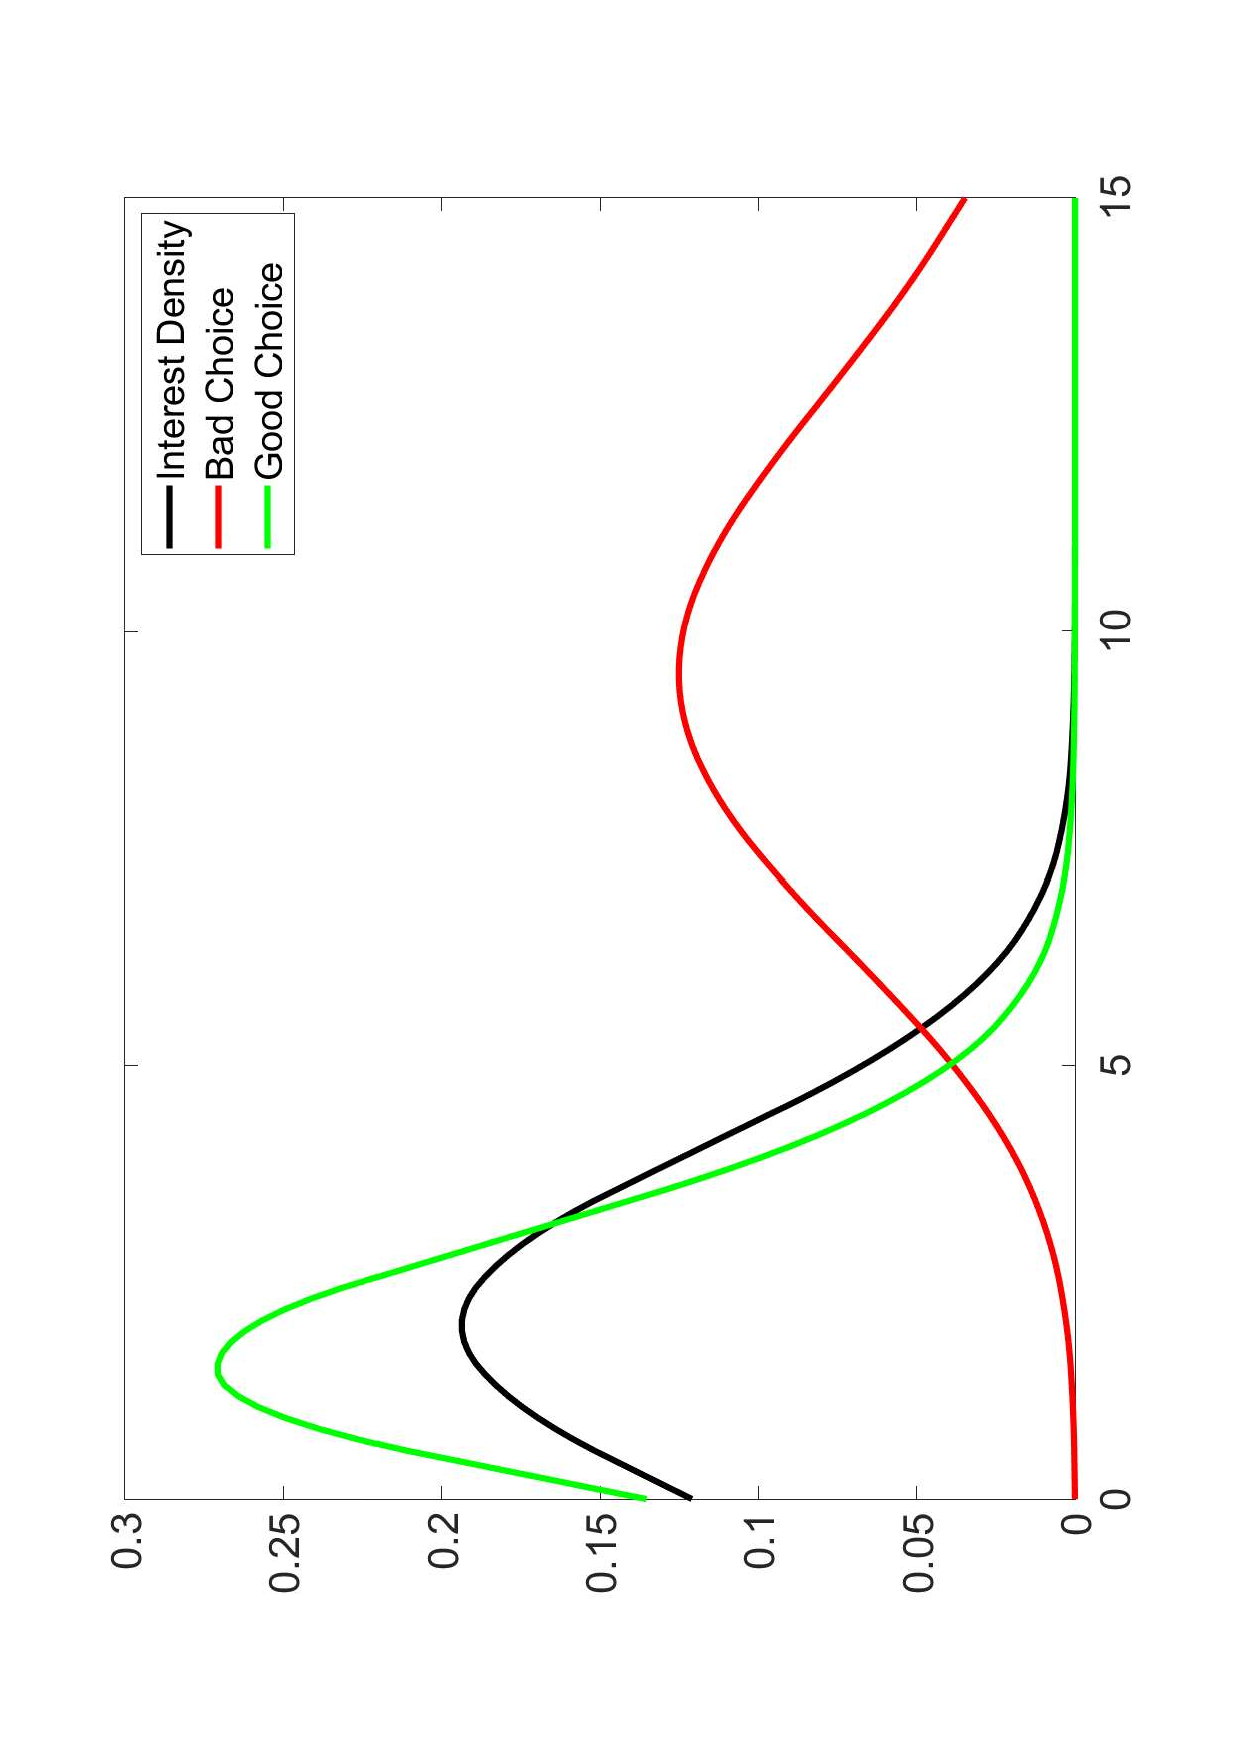
\includegraphics[scale = 0.3, angle=270]{Comparison.pdf}
           \caption{Good and Bad Choice of $q$ Density}
 \end{figure}

On the contrary, the bad choice of $q$ density will increase the variance.
\end{frame}

\begin{frame}{Example of Choosing $q$}

Now, let's use the likelihood ratio $w(\boldsymbol{x})=p(\boldsymbol{x}) / q(\boldsymbol{x})$ as a means to understand which importance sampling densities are good or bad choices. The first term in $\sigma_{q}^{2}$ is $\int f(x)^{2} p(x)^{2} / q(x) \mathrm{d} x$. Write the term as\\
\[\mathbb{E}_{p}\left(f(\boldsymbol{X})^{2} w(\boldsymbol{X})\right)=\mathbb{E}_{q}\left(f(\boldsymbol{X})^{2} w(\boldsymbol{X})^{2}\right)\]The appearance of $q$ in the denominator of $w$, means that light tailed importance densities $q$ are dangerous. One smart idea is that $f$ should be small just where it needs to be to offset the small denominator. However, we often need to use the same sample with multiple integral. \\
\textcolor{red}{So, as a rule, $q$ should have tails at least as heavy as $p$ does.}


\end{frame}

\begin{frame}{Example of Choosing $q$}

When $p$ is a Gaussian distribution, then a common tactic is to take $q$ to be a student's $t$ distribution. Such a $q$ has heavier tails than $p$. It even has heavier tails than $fp$ for integral of the form $f(\boldsymbol{x})=\exp \left(\boldsymbol{x}^{\top} \theta\right)$ (Proportional to another Gaussian density).\\
But, the reverse practice of using Gaussian importance distribution $q$ for a student's $t$ nominal distribution, can easily lead to $\sigma_{q}^{2}=\infty$. The infinite variance could be largely attributable to the unimportant region of $\mathcal{D}$ where $|f| p$ is small, where $q$ is extremely small.

\end{frame}

\begin{frame}{Importance Sampling}
\begin{block}{Importance Sampling Algorithm:}
\begin{itemize}
\item Draw $N$ samples from $q$.
\item Calculate the probability of each sample.
\item Evaluate $p$ over the N samples.
\item Calculate the importance weights $w=p / q$.
\item Draw $N$ samples from $g$ with new weight $w$.
\end{itemize}
\end{block}

\end{frame}

%%% Local Variables:
%%% mode: latex
%%% TeX-master: "probability-main"
%%% End:
